% tex file for hypothesis testing results

\begin{figure}[ht]

\centering

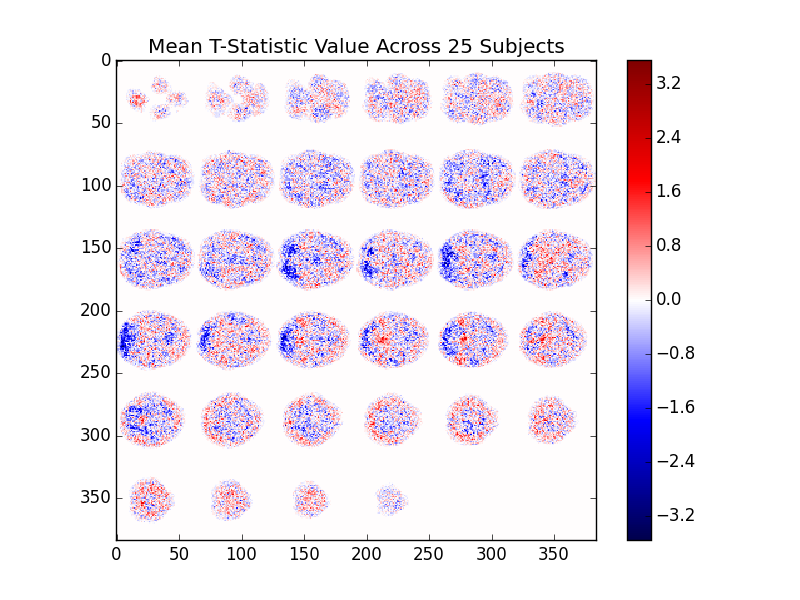
\includegraphics[scale=0.5]{images/hypothesis_testing}  

\caption{Across Subject Mean of T-Statistic Per Voxel}

\label{fig:mask}

\end{figure}


\par \indent The results of our t-statistic comparison is shown in [Figure \ref{fig:mask}]. we see each slice of the brain from top to bottom in each section of the image. The blue areas shows parts of the brain that had a negative t-statistic while the red parts of the image shows parts of the brain that had a positive t-statistic.

\par \indent The parts of the image that were cut out by the mask are white so we can more clearly see the contrast in our results. Based on a cursory look at this image, we can see a pattern of dark blue areas in the left middle parts of the brain, and area of dark red in the center middle parts parts of the brain. 


